\documentclass{article}
\usepackage{pgfplots}
\pgfplotsset{compat=1.18}

\begin{document}

\begin{figure}[htbp]
\centering
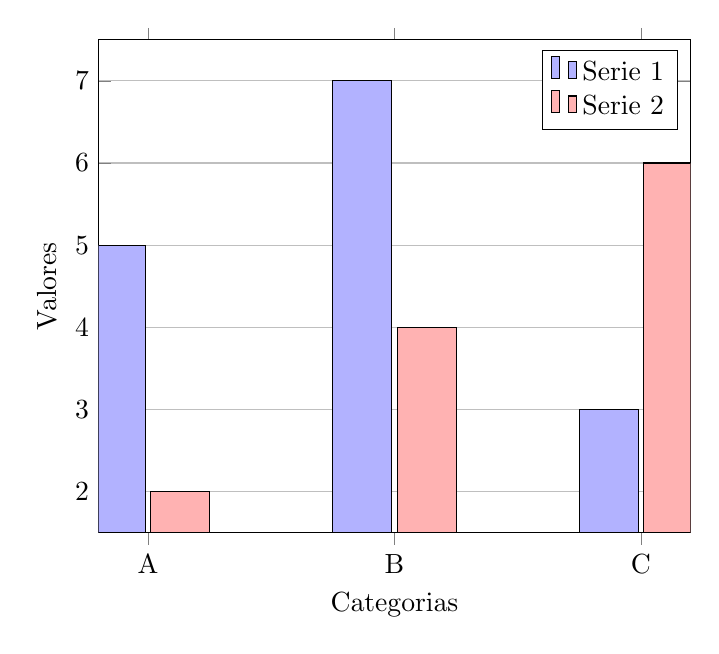
\begin{tikzpicture}
\begin{axis}[
    ybar,
    symbolic x coords={A,B,C},
    xtick=data,
    xlabel={Categorias},
    ylabel={Valores},
    width=0.75\textwidth,
    bar width=0.75cm,
    ymajorgrids=true
]
\addplot [fill=blue!30] coordinates {(A,5) (B,7) (C,3)};
\addplot [fill=red!30] coordinates {(A,2) (B,4) (C,6)}; % Segunda série de dados
\legend{Serie 1, Serie 2}
\end{axis}
\end{tikzpicture}
\caption{Gráfico de Barras Comparativo}
\label{fig:barras}
\end{figure}

\end{document}
